\documentclass[tikz,border=6pt]{standalone}
\usepackage{amsmath,amsfonts}

\usepackage{tikz}
\usepackage{graphicx}
\usepackage{xcolor}
\usetikzlibrary{
    arrows.meta,
    positioning,
    matrix,
    backgrounds,
    fit
}

\begin{document}

\begin{tikzpicture}[
    panel/.style={
        draw,
        rounded corners,
        align=center,
        inner sep=2mm
    },
    arr/.style={-{Stealth[length=3mm,width=2mm]}, thick}
]

\newcommand{\panelcaption}[1]{{\footnotesize\centering #1\par}}
\newlength{\imgw}
\setlength{\imgw}{4.0cm}

% --- Layout (avoid matrix-of-nodes parboxes) --------------------------
\node[panel, text width=4.5cm] (p1) {
    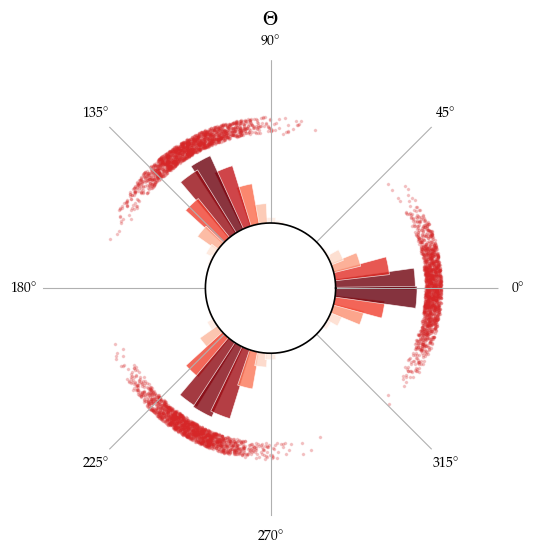
\includegraphics[width=\imgw]{tikz_S1_1_part1.png}\\[1mm]
    \panelcaption{\textbf{1} Latent variables $\Theta \sim G$}
};

\node[panel, text width=4.5cm, right=8mm of p1] (p2) {
    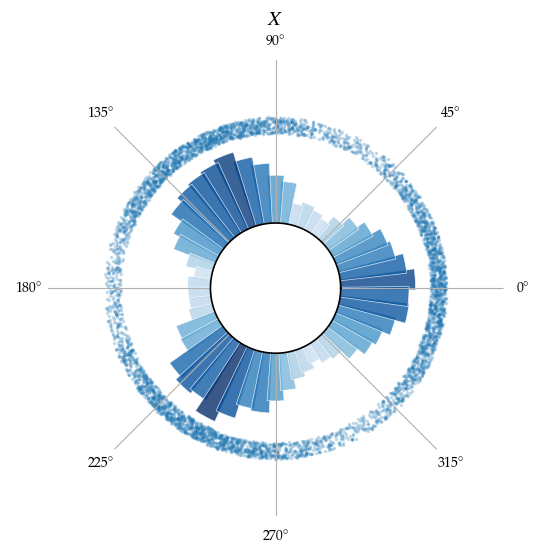
\includegraphics[width=\imgw]{tikz_S1_1_part2.png}\\[1mm]
    \panelcaption{\textbf{2} Measurements $X\sim \mathcal{N}(\Theta, \sigma^2)$}
};

\node[panel, text width=6.8cm, below=5mm of p2, anchor=north] (p34) {
    \centering
    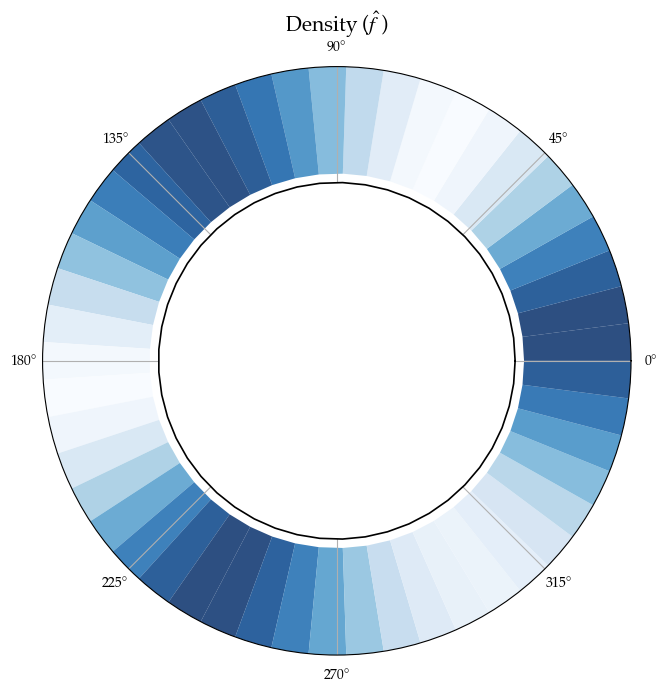
\includegraphics[width=0.78\imgw]{tikz_S1_2_part1.png}
    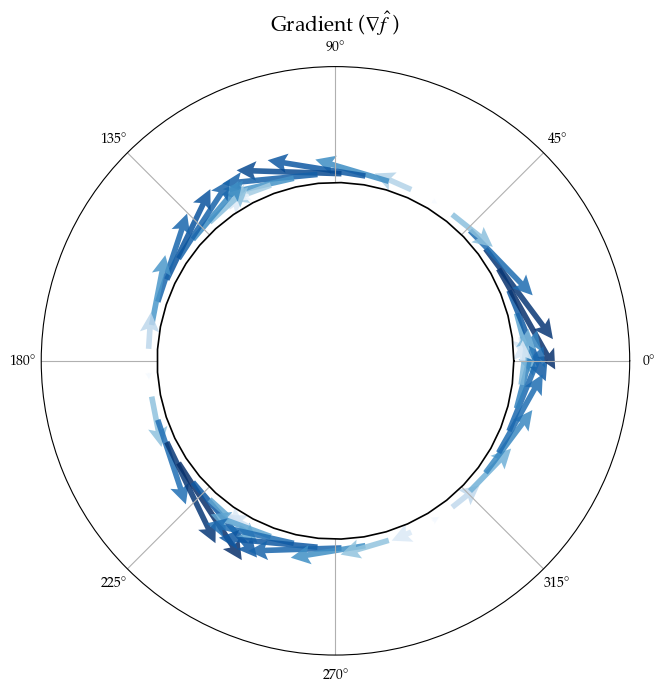
\includegraphics[width=0.78\imgw]{tikz_S1_2_part2.png}\\[1mm]
    \panelcaption{\textbf{3} Estimated marginal density $\hat f$ and gradient $\nabla \hat f$}\vspace{2mm}
    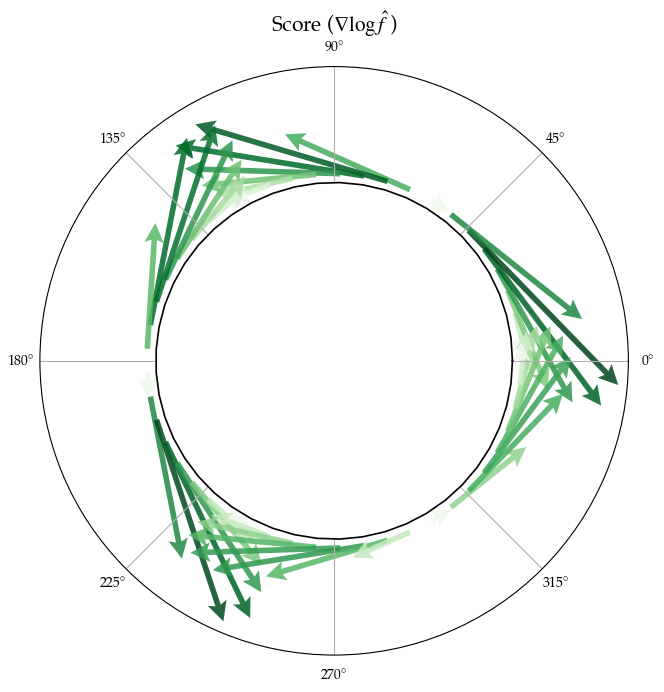
\includegraphics[width=\imgw]{tikz_S1_2_part3.png}\\[1mm]
    \panelcaption{\textbf{4} Estimated score field $\sigma^2 \nabla\log \hat f$}
};

\node[panel, text width=4.5cm, right=8mm of p34, yshift=0mm] (p5) {
    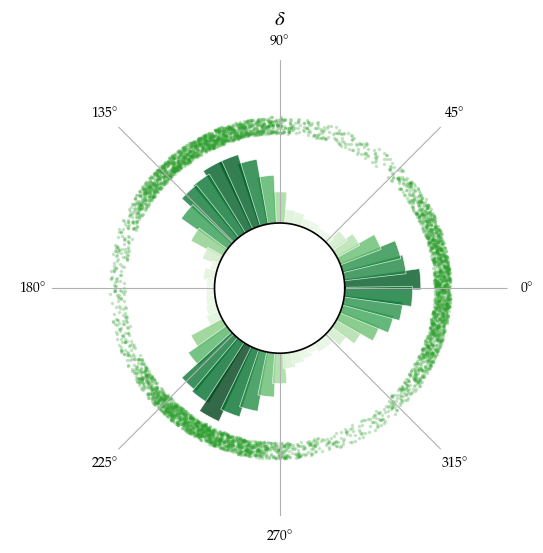
\includegraphics[width=\imgw]{tikz_S1_1_part3.png}\\[1mm]
    \panelcaption{\textbf{5} Denoised estimates $\delta(X)$}
};

% --- Arrows -----------------------------------------------------------
\draw[arr] (p1.east) -- (p2.west);
\draw[arr] (p2.south) -- (p34.north);
\draw[arr] (p34.east) -- (p5.west);

% --- Background highlight (merged estimation step) --------------------
\begin{pgfonlayer}{background}
    \node[
        fill=black!5,
        rounded corners,
        fit=(p34),
        inner sep=4mm
    ] {};
\end{pgfonlayer}

\end{tikzpicture}

\end{document}
